\documentclass[final]{beamer}

\mode<presentation>{
\usetheme{Bethlehem}
\usefonttheme[onlymath]{serif}
}
\usepackage{amsmath,amssymb,amsthm,fancyhdr,tikz,mathdots,bbm,tikz-cd,wrapfig,array,pigpen,enumerate,hyperref}
\usepackage[size=custom, width=121.9, height=91.44, scale=1.7]{beamerposter} %%%%Not final dims.


\newcommand{\fr}{\nobreak\mskip2mu\mathpunct{}\nonscript\mkern-\thinmuskip{:}\mskip3mu\relax}
\newcommand{\from}{\leftarrow}
\newcommand{\pathto}{\rightsquigarrow}
\newcommand{\inc}{\hookrightarrow}
\newcommand{\A}{\mathcal{A}}
\newcommand{\F}{\mathbb{F}}
\newcommand{\N}{\mathbb{N}}
\newcommand{\Z}{\mathbb{Z}}
\newcommand{\Sq}{\mathrm{Sq}}
\newcommand{\mm}{/\!/\!}

\newtheorem{lem}{Lemma}
\newtheorem{prop}{Proposition}
\newtheorem{thm}{Theorem}
\newtheorem{cor}{Corollary}
\newtheorem{defn}{Definition}
\newtheorem{ex}{Example}


\title{Determining the Structure of Length-$k$ Steenrod Operations as $A(r)$-Modules}
\author{Benjamin Kraft}
\institute{Massachusetts Institute of Technology}

\begin{document}

  \begin{columns}[T]
    \begin{column}{0.245\textwidth} %%% LEFT SIDE
      \begin{block}{Cohomology Operations} %explain quickly, including stable operations
        Let $H^n(X;R)$ be the $n$th degree cohomology of the space $X$ with coefficients in the ring $R$.
        \begin{bulletitem}
          A \alert{cohomology operation} is a natural transformation of cohomology functors, that is, for $m$ and $n$ and rings $R$ and $S$, a map $\Theta\fr H^n(X;R)\to H^m(X;S)$ for each $X$, such that the diagram below commutes for each $f\fr X\to Y$.
        \end{bulletitem}
        \begin{center}
          \vspace{-0.4em}
          \begin{tikzcd}
            H^m(Y;R) \arrow{r}{\Theta} \arrow{d}{f^*} & H^n(Y;S) \arrow{d}{f^*} \\
            H^m(X;R) \arrow{r}{\Theta}                & H^n(X;S)
          \end{tikzcd}
          \vspace{-0.4em}
        \end{center}
        \begin{bulletitem}
          A \alert{stable cohomology operation} of degree $i$ is a sequence of cohomology operations $\Theta\fr H^n(X;R)\to H^{n+i}(X;S)$ for each $n$ which commute with the suspension isomorphism $\Sigma$:
        \end{bulletitem}
        \begin{center}
          \vspace{-0.4em}
          \begin{tikzcd}
            H^n(X;R) \arrow{r}{\Theta} \arrow{d}{\Sigma} & H^{n+i}(X;S) \arrow{d}{\Sigma} \\
            H^n(\Sigma X;R) \arrow{r}{\Theta}            & H^{n+i}(\Sigma X;S)
          \end{tikzcd}
          \vspace{-0.4em}
        \end{center}
      \end{block}
      \subsection{The Steenrod Algebra}

      The \alert{Steenrod Algebra} $\A$ is the algebra of stable cohomology operations from $\Z/2$ cohomology to itself.  It is generated by operations $\Sq^i$ of degree $i$ such that:
      \begin{bulletitemize}
        \item $\Sq^0$ is the identity
        \item $\Sq^n(x)=x^2$ if $x\in H^n(X;\Z/2)$
        \item $\Sq^n(x)=0$ if $x\in H^m(X;\Z/2)$, $m<n$
        \item $\Sq^n(xy)=\displaystyle\sum_{i+j=k} \Sq^i(x)\Sq^j(y)$.
      \end{bulletitemize}
      The entire algebra consists of the $\Sq^i$ and their compositions, which satisfy the \alert{Adem relations}:
      \[ \Sq^i\Sq^j = \sum_{k=0}^{\lfloor i/2 \rfloor} \binom{j-k-1}{i-2k}\Sq^{i+j-k}\Sq^k .\]
      Using the Adem relations, we can write any element in terms of the $\Sq^{2^i}$.  We let \alert{$\A(r)$} be the subalgebra generated by the $\Sq^{2^i}$ for $i\leq r$.
    \end{column}
    \begin{column}{0.495\textwidth} %%% CENTER
      \section{Bases of the Steenrod Algebra}
      \begin{columns}[T]
        \begin{column}{0.497\textwidth}
          \begin{block}{Adem (Admissible)}
            Using the Adem relations, any product $\Sq^i\Sq^j$ may be rewritten if $i<2j$.  Then the \alert{Adem basis} consists of $\Sq^{i_1}\cdots\Sq^{i_k}$, $i_j \geq 2i_{j+1}$.
            We may define \alert{$L(k)$} to be the quotient of the Steenrod Algebra by the ideal generated by all Adem basis elements of length greater than $k$.
          \end{block}
        \end{column}
        \begin{column}{0.497\textwidth}
          \begin{block}{Milnor (Dual)}
            Milnor found that the Steenrod Algebra is a Hopf algebra, with a commutative comultiplication.  Thus the dual Steenrod Algebra is commutative, and in fact is a polynomial algebra over elements $\xi_n$.  The duals of the monomials $\xi_1^{i_1}\xi_2^{i_2}\cdots$, denoted $\Sq(i_1,i_2,\ldots)$, form the \alert{Milnor basis}.
          \end{block}
        \end{column}
      \end{columns}
      \vspace{0.2em}
      \begin{columns}[T]
        \begin{column}{0.497\textwidth}
          \begin{block}{$P^s_t$}
            Let $P^s_t=\Sq(0,0,\ldots,0,2^s)$, where the $2^s$ is in the $t$th position.  Pick any ordering on the pairs $(s,t)$; products of $P^s_t$ in that order constitute a basis.  The $P^s_t$ derives some convenient properties from the dual basis, while also giving some flexibility in the choice of ordering, allowing it to describe ideals nicely.
          \end{block}
        \end{column}
        \begin{column}{0.497\textwidth}
          \begin{block}{Wood $Z$}
            The element $P^s_t$ has degree $2^s(2^t-1)$.  If we replace it by $\Sq^{2^s(2^t-1)}$, and use the reverse left lexicographic ordering on $(s + t,s)$, we get an analogue of the $P^s_t$ basis which is monomial in the $\Sq^i$; it describes certain ideals nicely like the $P^s_t$ bases, but is closer to the Adem basis.  It consists of subproducts of $\cdots\Sq^4\Sq^6\Sq^7\Sq^2\Sq^3\Sq^1$.
          \end{block}
        \end{column}
      \end{columns}
      \begin{section}{Structure of the Subalgebras}
        \begin{columns}[T]
          \begin{column}{0.33\textwidth}
            Welcher showed that $L(k)$ is a free $\A(k-1)$-module, so it is natural to consider the structure of $L(k)$ as an $\A(r)$-module for any $r$.  In particular, it appears that $L(k)$ is built up out of the ``quotient'' algebras $\A(r)\mm\A(r-k)$ (see below).
            \begin{block}{$\A(r)\mm\A(r-k)$}
              Consider $\A(r)$ as an $\A(r-k)$-module; note that we may also consider $\F_2$ to be an $\A(r-k)$-module, where the action of any element except $1$ is zero.  Then we may define \alert{$\A(r)\mm\A(r-k)$} to be the tensor algebra $\A(r)\otimes_{\A(r-k)}\F_2$.
              \begin{bulletitem}
                \alert{Intuitively}, $\A(r)\mm\A(r-k)$ is like $\A(r)$, but with any element which can be written as a product ending in $\Sq^{2^i}$, $i\leq r-k$, equal to zero.
              \end{bulletitem}
            \end{block}
          \end{column}
          \begin{column}{0.66\textwidth}
            \begin{block}{Small $\A(r)$}
              \begin{wrapfigure}{r}{4.2in}
                \vspace{-0.8em}
                \begin{center}
                  \hspace{-0.7in}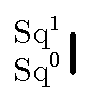
\includegraphics[scale=2]{pics/A0.pdf}\\[1em]
                  \hspace{-0.7in}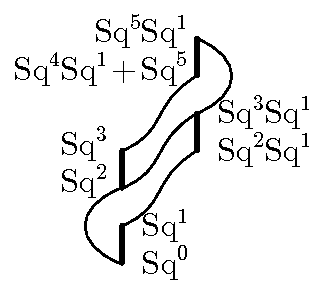
\includegraphics[scale=2]{pics/A1.pdf}
                  \vspace{0.2em}
                \end{center}
              \end{wrapfigure}
              $\A(0)$ is simple: it is spanned by $\Sq^0=1$ and $\Sq^1$, with $\Sq^1\Sq^1=0$.  It is shown as an $\A(0)$-module above right.  Each point represents an element of the (Adem) basis, and the thick solid line represents the (left) action of $\Sq^1$ (in this case, on $1$).  To represent an $\A(1)$ module, we use a thinner curved line for the (left) action of $\Sq^2$; $\A(1)$ is shown below right. So we know $\Sq^1\Sq^2=\Sq^3$ and $\Sq^2\Sq^3=\Sq^4\Sq^1+\Sq^5$.
            \end{block}
            \begin{wrapfigure}{R}{2in}
              \begin{center}
                \vspace{-1em}
                \hspace{-0.5in}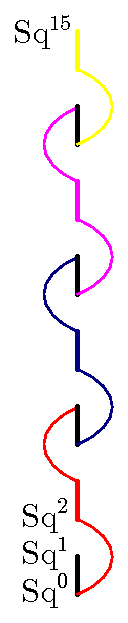
\includegraphics[scale=2]{pics/L1-1.pdf}
              \end{center}
            \end{wrapfigure}
            \subsection{$L(1)$}
            \parbox{0.85\textwidth}{
              \begin{wrapfigure}{R}{2.5in}
                \begin{center}
                  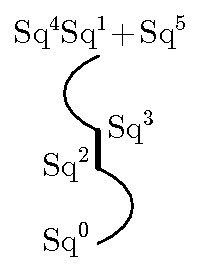
\includegraphics[scale=2]{pics/A1-A0.pdf}
                \end{center}
              \end{wrapfigure}

              On the far right is shown the small-degree classes of $L(1)$ as an $\A(1)$-module; it continues periodically upwards.  Looking only at the thick lines, as an $\A(0)$-module, it is indeed free, with basis $\Sq^{2i}$.  As an $\A(1)$-module, it is not free, but it is still built up out of copies of $\A(1)\mm\A(0)$ (shown near right), in the sense that it has a filtration in which the filtration quotients are isomorphic to $\A(1)\mm\A(0)$, except for one containing only the single class $\Sq^0$.
            }
          \end{column}
        \end{columns}
      \end{section}
    \end{column}
    \begin{column}{0.245\textwidth} %%% RIGHT SIDE
      \vspace{1em}
      \subsection{$L(2)$}\\
      \begin{wrapfigure}{l}{6.3in}
        \begin{center}
          \vspace{-1em}
          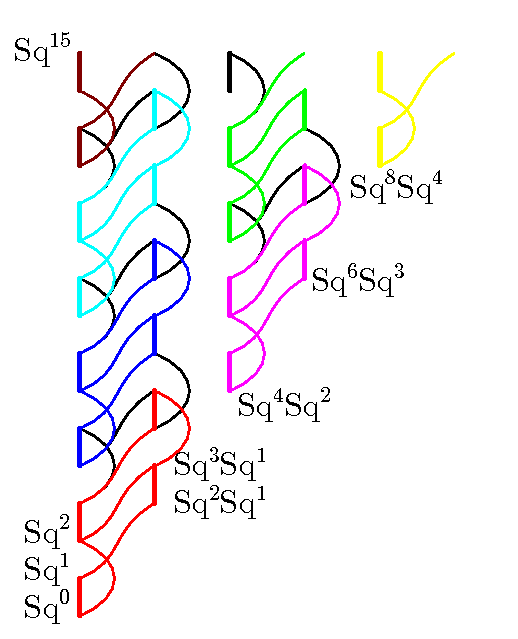
\includegraphics[scale=2]{pics/L2-1.pdf}
          \vspace{-1em}
        \end{center}
      \end{wrapfigure}
      At right is shown $L(2)$ as a free module over $\A(1)$, as Welcher showed.  We can show that, indeed, $L(2)$ considered as an $\A(2)$ module has a filtration with filtration quotients in each dimension isomorphic to $\A(2)\mm\A(0)$, with the exception of a single class in every dimension, and a finite number of extra classes.

      \begin{block}{The general case}
        In the general case, we have shown, essentially, that the filtration exists, but not that it covers all of $L(k)$.  In particular, we prove the commutation identity that, if we let
        \[X_n = \Sq^{2^{n+1}-2^n}\Sq^{2^{n+1}-2^{n-1}}\cdots\Sq^{2^{n+1}-1},\]
        then
        \[X_nX_{n-1}\Sq^{2^{n+1}m} = X_n\Sq^{2^{n+1}m}X_{n-1}.\]
        This allows us to show that the top class $X_rX_{r-1}\cdots X_{r-k+1}$ of $\A(r)\mm\A(r-k)$, when multiplied by the basis elements $\Sq^{2^{r+1}m_1}\Sq^{2^rm_2}\cdots\Sq^{2^{r-k+2}m_k}$ for $m_1\geq m_2\geq\cdots m_{r-k}$, produces a linearly independent set.

        We hope to show that these filtrations in fact cover all but some set of classes which has, in the natural sense, lower dimensionality than $L(k)$; so far we have been able to show this only in specific cases, by finding the actual set of excluded classes in each case, but we hope to soon complete the general result.
      \end{block}
      \subsection{Acknowledgements}

      This project would not have been possible without the support of Mark Behrens, who proposed the problem and provided guidance along the way, and funding from the MIT Class of 1995 and Paul E. Gray Funds for UROP.

    \end{column}
  \end{columns}
\end{document}

